\section*{Введение}

Этап поддержки и сопровождения в жизненном цикле программного обеспечения может занимать до 90\% времени существования программного продукта. На этом этапе особенно важно понимание программного текста поддерживаемой системы, что зачастую бывает сложной задачей. Необходимым условием для лучшего понимания программного текста является его аккуратное оформление, отражающее структуру%(ы)
программы. Существуют различные стандарты оформления кода (стили кодирования) -- наборы правил и соглашений, используемые при написании исходного кода на некотором языке программирования.
Рассмотрим их на примере стандарта кодирования, принятого в компании Google\footnote{\texttt{https://google-styleguide.googlecode.com/svn/trunk/cppguide.html}}, и стандарта, используемого в проекте GNU\footnote{\texttt{http://www.gnu.org/prep/standards/standards.html}} (см. рис ~\ref{codingstandards}) для языка C++.


\fvset{frame=lines,framesep=7pt}
\begin{figure}[ht]
\noindent\begin{minipage}{.5\textwidth}
    \lstinputlisting[language=C++]{codes/exGoogleCC.txt}
\caption*{а) Стиль кодирования Google}    
\end{minipage}\hfill
\begin{minipage}{.5\textwidth}
    \lstinputlisting[language=C++]{codes/exGNUCC.txt}
\caption*{б) Стиль кодирования GNU}    
\end{minipage}
\caption{Различные стили кодирования для языка С++}    
\label{codingstandards}
\end{figure}

Когда программист работает над проектом, он придерживается некоторого стиля кодирования. 
Если файлы проекта с одним стилем кодирования присоединяется к уже существующему проекту с другим стилем кодирования, то их форматирование нужно привести к тому же виду. 
Для решения этой задачи можно воспользоваться уже существующими средствами, например, форматтерами (программами, которые форматируют исходный текст) в IDE таких, как Eclipse, IntelliJ IDEA, Visual Studio и др. 
Однако в этом случае необходимо вручную задавать настройки форматирования.
Кроме того, количество принципиально разных стилей форматирования, которые можно задать с помощью данных настроек, невелико.

%Однако в этом случае необходимо иметь настройки форматирования, заданные программистом, но в целом, количество принципиально разных стилей форматировани, которые можно задать с помощью данных настроек, невелико. %причем эти настройки могут быть различными в разных IDE.
% * <Anton Podkopaev> 12:15:51 22 May 2015 UTC+0300:
% Нужно переработать это предложение.

Еще одним примером может послужить принтер-плагин для IntelliJ IDEA\cite{podkopaev:diploma}, который позволяет форматировать исходный код проекта по образцу. 
В качестве образца используется код из некоторого репозитория. 
Из него выделяются шаблоны форматирования для структур языка, которые применяются к структурам целевого кода. 
Под \textit{шаблоном} понимаются данные, сопоставление которых с элементом синтаксического дерева дает текстовое представление этого элемента (и его потомков). 
Например, на рис.~\ref{fig:ifTree} представлено дерево разбора для оператора ветвления. 


\begin{figure}[h]
	\centering
	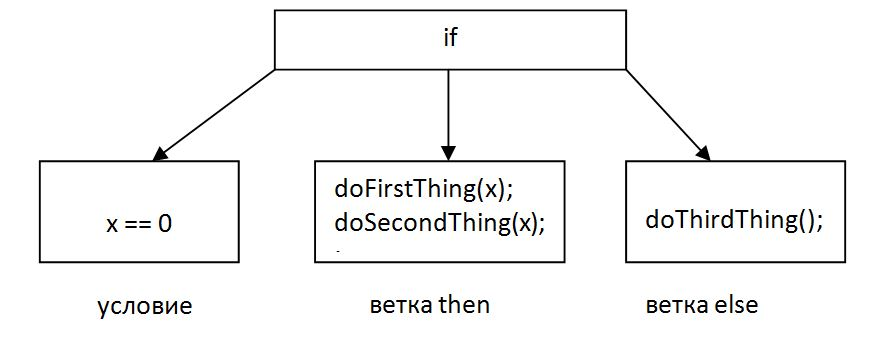
\includegraphics[width=\textwidth]{images/ifTree.jpg}
	\caption{Представление оператора ветвления в виде дерева разбора}
	\label{fig:ifTree}
\end{figure}

На рис.~\ref{fig:tmpltcodeintro}а изображен шаблон форматирования, который может быть применен к нему (несколько подвыражений, соответствующих выполнению условия, и одно подвыражение, соответствующее невыполненению условия).
На рис.~\ref{fig:tmpltcodeintro}б представлен результат применения этого шаблона к дереву разбора для оператора ветвления.

% \begin{figure}[h]
% 	\centering
% 	\lstinputlisting[language=c++]{codes/ifTmpltIntro.txt}
% 	\caption{Шаблон для оператора ветвления}
% 	\label{fig:ifTmpltIntro}
% \end{figure}

% На рис.~\ref{fig:ifCodeIntro} представлен результат применения этого шаблона к дереву разбора для оператора ветвления.

% \begin{figure}[h]
% 	\centering
% 	\lstinputlisting[language=c++]{codes/ifCodeIntro.txt}
% 	\caption{Представление дерева разбора при применении шаблона}
% 	\label{fig:ifCodeIntro}
% \end{figure}


\fvset{frame=lines,framesep=7pt}
\begin{figure}[ht]
\noindent\begin{minipage}{.5\textwidth}
    \lstinputlisting[language=C++]{codes/ifTmpltIntro.txt}
\caption*{а) Шаблон для оператора ветвления}    
\end{minipage}\hfill
\begin{minipage}{.5\textwidth}
    \lstinputlisting[language=C++]{codes/ifCodeIntro.txt}
\caption*{б) Текст, полученный при применении шаблона к дереву разбора}    
\end{minipage}
\caption{Оператор ветвления и шаблон для него}    
\label{fig:tmpltcodeintro}
\end{figure}

Однако не всегда этот репозиторий существует. Кроме того, необходимо наличие заданного форматирования для всех структур языка.
% * <Anton Podkopaev> 12:19:02 22 May 2015 UTC+0300:
% 'Однако не всегда удобно иметь этот репозиторий под рукой.' --- поменять. Не про удобство надо говорить.

Шаблоны можно извлекать из уже существующего кода и применять их к другим элементам того же типа, но отформатированных иным способом. 
Например, пользователь меняет форматирование некоторой структуры языка (в частности, оператор ветвления), программа извлекает из полученного участка кода новый шаблон и применяет его к структурам того же типа, содержащим старое форматирование. 
Назовем такой способ задания шаблонов -- форматирование в режиме
онлайн.
%картинки

Целью данной работы является расширение функциональности описанного 
принтер-плагина путем добавления возможности задания шаблонов в режиме онлайн. 